\begin{figure}[H]
\centering
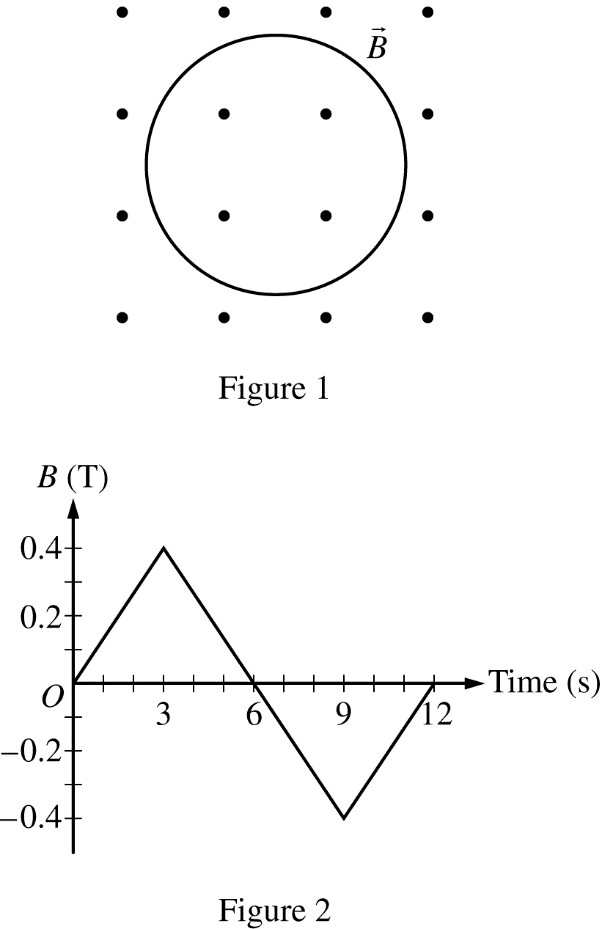
\includegraphics[scale=0.4]{images/img-015-022.png}
\end{figure}

% Multiple Choice Question 33
\begin{questions}\setcounter{question}{32}\question
A metal wire of resistance $10 \latinunit\Omega$ is bent into a circular hoop of radius $0.10$ meter and placed in a uniform magnetic field, as shown in Figure 1 above. The magnetic field strength $B$ as a function of time is shown in Figure 2, where positive refers to a magnetic field directed out of the page. What are the magnitude and direction of the current induced in the ring at time $t=6 \unit{s}$ ?

\tabto{0.75cm}\underline{Magnitude}
\tabto{4.00cm}\underline{Direction}

\begin{choices}
\choice $3.8  \unit{mA}$ \tabto{3.25cm} Clockwise
\choice $3.8  \unit{mA}$ \tabto{3.25cm} Counterclockwise
\choice $0.42 \unit{mA}$ \tabto{3.25cm} Clockwise
\choice $0.42 \unit{mA}$ \tabto{3.25cm} Counterclockwise
\choice Zero             \tabto{3.25cm} No direction
\end{choices}\end{questions}
